% This is a model template for the solutions in computational science. You can find a very useful documentation for LaTeX in Finnish at ftp://ftp.funet.fi/pub/TeX/CTAN/info/lshort/finnish/ or in English at ftp://ftp.funet.fi/pub/TeX/CTAN/info/lshort/english/. The section List of mathematical symbols in Chapter 3 is especially useful for the typesetting of mathematical formulas.

% Compile the document to PDF by command 'pdflatex model.tex' in the terminal. The command must be run twice for the references in the text to be correct.

\documentclass[a4paper,11pt]{article}
\usepackage[utf8]{inputenc}
% This includes letters such as � and �
\usepackage[T1]{fontenc}
% Use here 'Finnish' for Finnish hyphenation. You may have to compile the code twice after the change. 
\usepackage[english]{babel}
\usepackage{graphicx}
% Some math stuff
\usepackage{amsmath,amsfonts,amssymb,amsbsy,commath,booktabs}  
% This is just to include the urls
\usepackage{hyperref}
\usepackage[margin=2cm]{geometry}

\setlength{\parindent}{0mm}
\setlength{\parskip}{1.0\baselineskip}

\usepackage{listings}
\usepackage{color}

\definecolor{dkgreen}{rgb}{0,0.6,0}
\definecolor{gray}{rgb}{0.5,0.5,0.5}
\definecolor{mauve}{rgb}{0.58,0,0.82}

\lstset{frame=tb,
	language=Python,
	aboveskip=3mm,
	belowskip=3mm,
	showstringspaces=false,
	columns=flexible,
	basicstyle={\small\ttfamily},
	numbers=none,
	numberstyle=\tiny\color{gray},
	keywordstyle=\color{blue},
	commentstyle=\color{dkgreen},
	stringstyle=\color{mauve},
	breaklines=true,
	breakatwhitespace=true,
	tabsize=4
}

\begin{document}

\title{Becs-114.1100 Computational Science -- exercise round 2} % Replace the exercise round number
\author{Kunal Ghosh, 546247} % Replace with your name and student number
\maketitle
\section{Solution to Question 2 (a)}\label{prob2a}

\begin{center}
	\begin{table}[h!]
		\begin{tabular}{|c|c|c|c|}
			\hline
			& \textbf{$x_n$} & \textbf{$f(x_n)$} & \\
			\hline
			& 0.57735 & -5.38490017946 & \\
			& -5774691.30483 & -1.92568975495e+20 & \\
			& -3849794.20322 & -5.70574742208e+19 & \\
			& -2566529.46881 & -1.69059182876e+19 & \\
			& -1711019.64587 & -5.00916097411e+18 & \\
			& -1140679.76392 & -1.48419584418e+18 & \\
			& -760453.175945 & -4.39761731609e+17 & \\
			& -506968.783963 & -1.30299772329e+17 & \\
			& -337979.189309 & -3.86073399492e+16 & \\
			& -225319.45954 & -1.14392118368e+16 & \\
			& -150212.973028 & -3.38939609977e+15 & \\
			& -100141.98202 & -1.00426551103e+15 & \\
			& -66761.3213489 & -2.97560151409e+14 & \\
			& -44507.5475693 & -8.8165970783e+13 & \\
			& -29671.6983845 & -2.61232505991e+13 & \\
			& -19781.1322638 & -7.74022239752e+12 & \\
			& -13187.4215204 & -2.29339922743e+12 & \\
			& -8791.6143638 & -6.79525696041e+11 & \\
			& -5861.07626779 & -2.01340946325e+11 & \\
			& -3907.38421639 & -59656576256.1 & \\
			& -2604.92286769 & -17676022306.3 & \\
			& -1736.61533019 & -5237339750.94 & \\
			& -1157.74368087 & -1551804243.31 & \\
			& -771.829311282 & -459793765.406 & \\
			& -514.553159306 & -136235133.874 & \\
			& -343.035865117 & -40365928.7734 & \\
			& -228.691210394 & -11960251.0783 & \\
			& -152.461746781 & -3543762.45335 & \\
			& -101.642550399 & -1049993.69253 & \\
			& -67.7637253191 & -311103.009159 & \\
			& -45.1787335034 & -92174.945674 & \\
			& -30.1232585281 & -27309.0439797 & \\
			& -20.0877147577 & -8090.63230212 & \\
			& -13.3987478053 & -2397.030783 & \\
			& -8.93981373361 & -710.532509955 & \\
			& -5.96389606269 & -211.160294544 & \\
			& -3.96624263936 & -63.427040294 & \\
			& -2.59316212981 & -19.8445302435 & \\
			& -1.558162687 & -7.22485525043 & \\
			& -0.40836950412 & -4.65973250245 & \\
			& -9.73337273448 & -917.392196014 & \\
			& -6.49417233487 & -272.392833164 & \\
			& -4.32410615269 & -81.5275724202 & \\
			& -2.84430721072 & -25.1663756491 & \\
			& -1.76282441275 & -8.71524043281 & \\
			& -0.715653053283 & -4.65087530829 & \\
			& 7.95362390822 & 490.193684532 & \\
			& 5.35698948537 & 143.37433958 & \\
			& 3.67205642057 & 40.841946317 & \\
			& 2.63682496403 & 10.6966126523 & \\
			\hline
			\end{tabular}
			\caption{ Table logging the Newton's approximation of $x_n$, $f(x_n)$ at each iteration. }
			\label{table:1}
		\end{table}
	\end{center}
	
\begin{figure}[h]
	\centering
	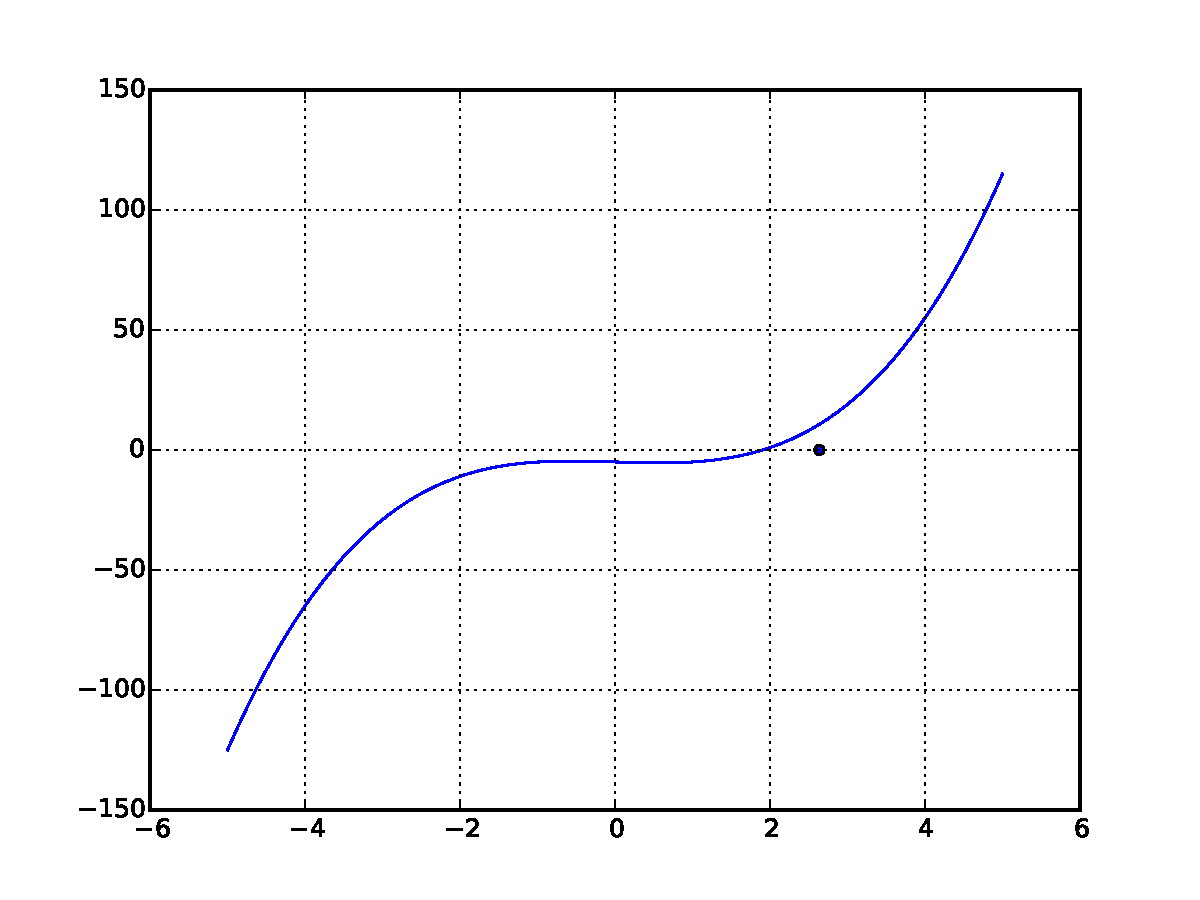
\includegraphics[scale=0.45]{solution2a_fig.pdf}
	\caption{The graph is the function $x^3 - x - 5 = 0$ and the point is the value of $x_n$ Newton's method converged to after 50 iterations.}
	\label{fig:solution2a_fig}
\end{figure}
	
It can be observed from the table of $x_n$ and $f(x_n)$ that initially the root found by newton's method goes to really large values very far away from the actual root. This is because we hit the "Flat Spot" at that point where the slope $f'(x)$ is almost zero which means $\frac{1}{f'(x)}$ becomes really large and when we subtract that from $x_n$ we get really large approximation which might throw us far away from the actual root.

The corresponding python code can be found at \ref{code:problem2a}
\clearpage

\section{Solution to Question 2 (b)}\label{prob2b}

In the solution to this problem I arbitrarily chose bounds of -5 and +5 for the bisection method. Then everytime, the $x_n$ from newton method went out of bounds, I used bisection method and updated the bounds of the bisection method, as can be seen in the table below. The number of steps taken to converge to the root reduced drastically !

\begin{center}
	\begin{table}[h!]
		\begin{tabular}{|c|c|c|c|c|c|}
			\hline
			& \textbf{Method} & \textbf{New $x$} & \textbf{$F(x)$} & \textbf{Comments} & \\
			\hline
			& Newton & -5774691.30482718 & -1.925689754950669e+20 & - & \\
			\hline
			& Bisection & 0.0 & -5.0 & new bisec min = 0.0  max =5 & \\
			\hline
			& Newton & -5.0 & -125.0 & - & \\
			\hline
			& Bisection & 2.5 & 8.125 & new bisec min = 0.0 max = 2.5 & \\
			\hline
			& Newton & 2.0422535211267605 & 1.475576330428514 & - &\\
			\hline
			& Newton & 1.914080721014927 & 0.09854639952939426 &- & \\
			\hline
			& Newton & 1.904217317447332 & 0.0005576843842707291 & - &\\
			\hline
			& Newton & 1.904160860978299 & 1.820794359730371e-08 & - &\\
			\hline
			& Newton & 1.9041608591349206 & 0.0 & - &\\
			\hline
			& Newton & 1.9041608591349206 & 0.0 & - &\\
			\hline
		\end{tabular}
		\caption{ Table logging the approximation technique used, $x_n$, $f(x_n)$ and few other values at each iteration.}
		\label{table:2}
	\end{table}
\end{center}

\begin{figure}[h]
\centering
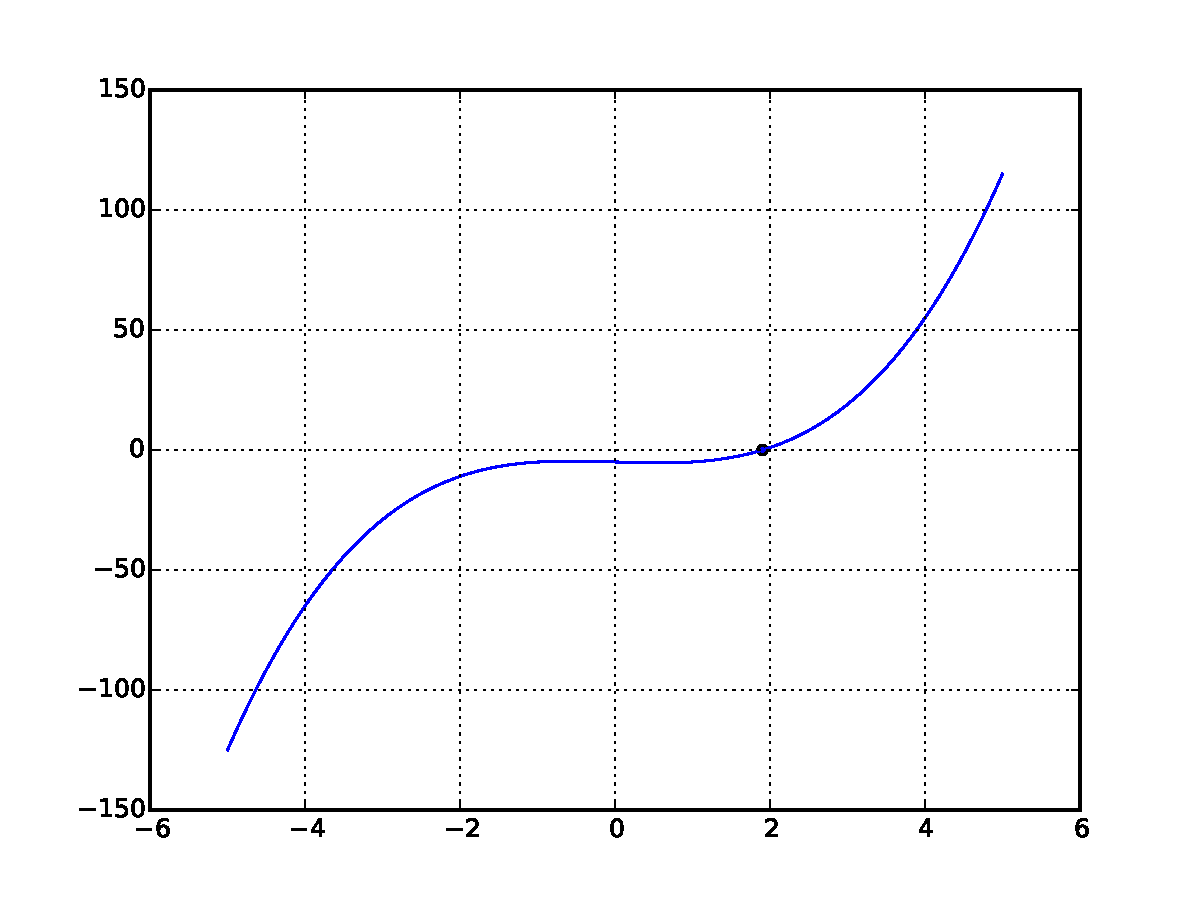
\includegraphics[scale=0.45]{solution2b_fig.pdf}
\caption{Plot of the function $x^3 - x - 5 = 0$ and our approximated root $x_n$ plotted by the point.}
\label{fig:solution2b_fig}
\end{figure}

The corresponding python code can be found at \ref{code:problem2b}
\clearpage

\section{Solution to Question 3}\label{prob3}

This problem is essentially the same as the second question. The only difference is that the new functions must handle compelx numbers instead of real values.

Note : Early stopping of iteration is really important and I noticed it in this problem since my first draft of the code did not have the stopping criterion and the plot for 1000 points took a really really long time ( maybe around 7 hours, I ran it overnight ). 

\begin{figure}[h]
	\centering
	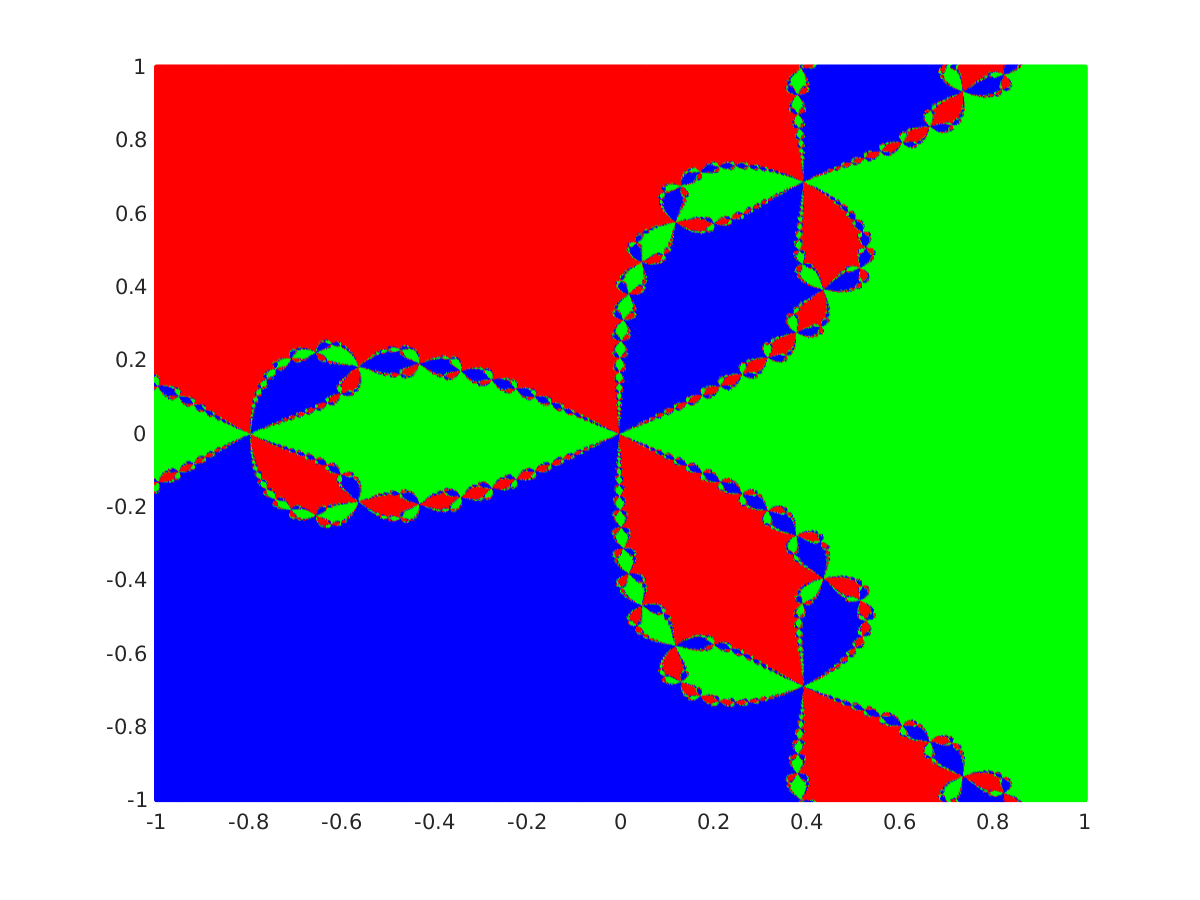
\includegraphics[scale=0.45]{Basin_1000.png}
	\caption{Basin of attraction with Real values on X axis and Imaginary values on the Y scale for $z^3 - 1 = 0$  Green is $(-1,0j)$ , Red is $(-5, -0.866j)$ and Blue is $(-5, 0.866j)$}
	\label{fig:basin1000}
\end{figure}

\begin{figure}[h]
	\centering
	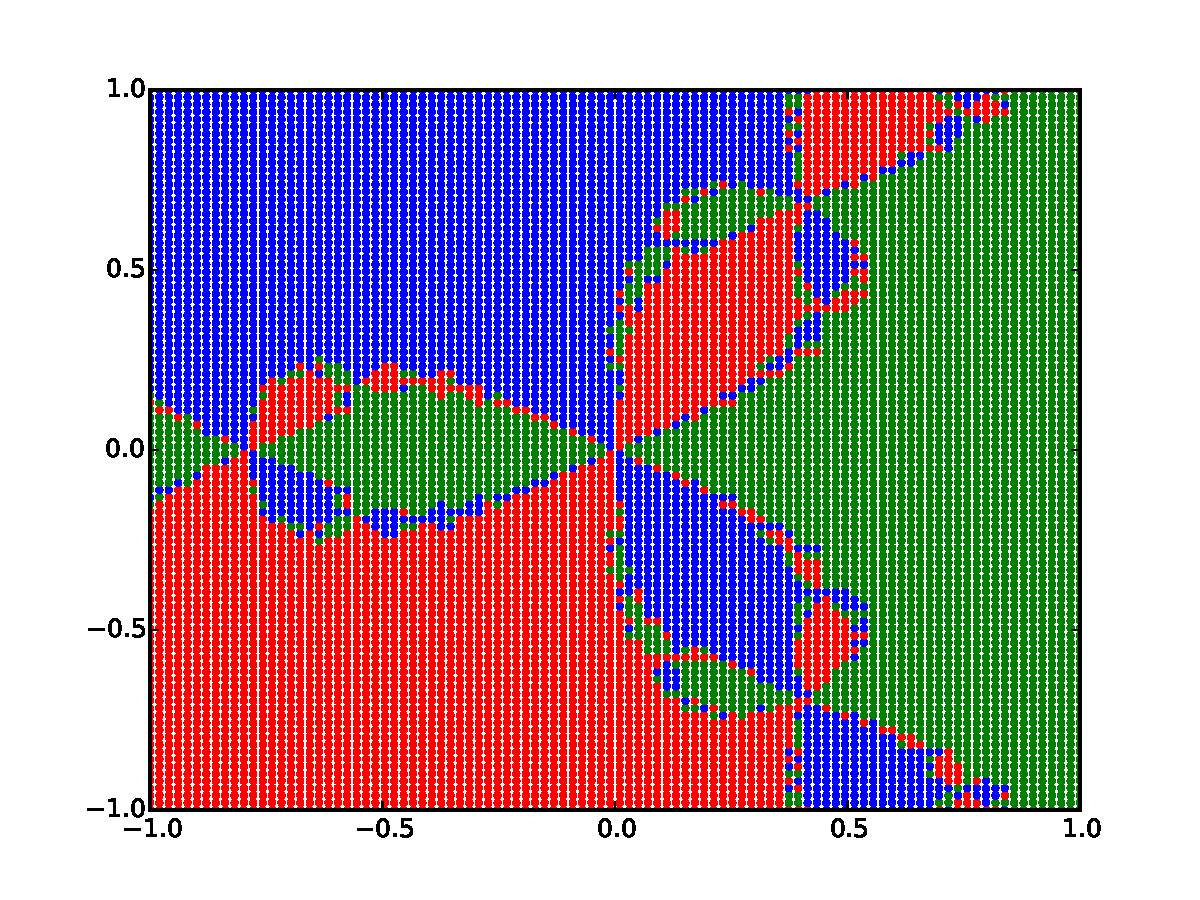
\includegraphics[scale=0.45]{figure_q3_new.pdf}
	\caption{Basin of attraction plotted for 100 values each, on X and Y axes. Real values on X axis and Imaginary values on the Y scale for $z^3 - 1 = 0$  Green is $(-1,0j)$ , Red is $(-5, -0.866j)$ and Blue is $(-5, 0.866j)$}
	\label{fig:basin100}
\end{figure}


The corresponding python code can be found at \ref{code:problem3}

\clearpage
%\ldots

\section{Appendix A}\label{code:problem2a}
Python source code for \ref{prob2a}.
{\footnotesize
\begin{lstlisting}
from __future__ import division
import doctest
import pylab as pl
import numpy as np
# use newton's method to calculate roots
# equation = x^3 - x - 5
# x_initial = 0.57735
# max_iter = 50
# print the results and explain them

## TODO : Write tests
# x^3 - x - 5 , re-written to get rid of powers
def f(x):
	'''
	>>> f(1)
	-5
	>>> f(2)
	1
	>>> f(3)
	19
	'''
	return (x * (x+1) * (x-1)) - 5

# 3 x^2 - 1 , re-written to get rid of powers
def f_dash(x):
	'''
	>>> f_dash(1)
	2
	>>> f_dash(2)
	11
	'''
	return (3 * (x + 1) * (x - 1)) + 2


def get_next_appox(x_n_minus_1):
	x = x_n_minus_1
	return x - (f(x) / f_dash(x))

if __name__ == '__main__':
	doctest.testmod()
	x_n_minus_1 = 0.57735 # x_initial
	# iterate for a maximum of 50 iterations
	max_iter = 50
	output = []
	for _ in xrange(max_iter):
		x_n = get_next_appox(x_n_minus_1)
		output.append((x_n_minus_1, f(x_n_minus_1)))
		x_n_minus_1 = x_n
	
	for val in output:
		print val
	
	# plot the curve
	pl.figure(1)
	x = np.linspace(-5,5,1000)
	y = [f(_) for _ in x]
	
	pl.grid(True)
	pl.plot(x,y)
	pl.scatter(output[-1][0],0)
	
	pl.savefig("solution2a_fig.pdf")
	pl.show()
\end{lstlisting}
}



\clearpage
\section{Appendix B}\label{code:problem2b}
Python source code for \ref{prob2b}.
{\footnotesize
\begin{lstlisting}
from __future__ import division
import doctest
import pylab as pl
import numpy as np
# a)	use newton's method to calculate roots
# 		equation = x^3 - x - 5
#		x_initial = 0.57735
#		max_iter = 50
#		print the results and explain them


# x^3 - x - 5 , re-written to get rid of powers
def f(x):
	'''
	>>> f(1)
	-5
	>>> f(2)
	1
	>>> f(3)
	19
	'''
	return (x * (x+1) * (x-1)) - 5

# 3 x^2 - 1 , re-written to get rid of powers
def f_dash(x):
	'''
	>>> f_dash(1)
	2
	>>> f_dash(2)
	11
	'''
	return (3 * (x + 1) * (x - 1)) + 2

def is_within_bound(val, lower, upper):
	returnVal = False
	# Checks for strict bounds
	if val >= lower and val <= upper:
		returnVal = True
	return returnVal

def get_next_approx_newton(x_n_minus_1):
	x = x_n_minus_1
	return x - (f(x) / f_dash(x))

def get_next_approx_bisection(func, b_min, b_max):
	# returns the new approx root of func
	# via bisection method, new lower and upper bounds
	mid = 0.5 * (b_min + b_max)
	new_b_min = b_min
	new_b_max = b_max
	if (func(new_b_min) * func(mid) < 0):
		new_b_max = mid
	elif (func(mid) * func(new_b_max) < 0):
		new_b_min = mid
	return mid, new_b_min, new_b_max

if __name__ == '__main__':
	doctest.testmod()
	x_n_minus_1 = 0.57735 # x_initial
	# iterate for a maximum of 50 iterations
	max_iter = 50
	# Bounds for bisection method.
	# Assuming [-5, 5] arbitrarily and it also satisfies
	# f(-5) * f(5) < 0
	bisection_min, bisection_max = -5, 5
	
	# run till new root approximation and old root approximation
	# are not same upto the given precision
	tolerance = 0.0000000001
	
	# first approximation from newton's method to setup the while loop
	x_n = get_next_approx_newton(x_n_minus_1)
	print ["method", "New x", "f(x)"]
	print ["newton", x_n, f(x_n)]
	
	while abs(x_n - x_n_minus_1) > tolerance:
		x_n_minus_1 = x_n
		if is_within_bound(x_n, bisection_min, bisection_max):
			# if the root is within bounds then use newton's method
			x_n = get_next_approx_newton(x_n_minus_1)
			print ["newton", x_n, f(x_n)]
		else:
			# else use bisection method
			x_n, bisection_min, bisection_max = get_next_approx_bisection(f, bisection_min, bisection_max)
			print ["bisection", x_n, f(x_n), "new bisec min = ", bisection_min, "new bisec max = ", bisection_max]
		
	pl.figure(1)
	# plot the curve
	x = np.linspace(-5,5,1000)
	y = [f(_) for _ in x]
	pl.grid(True)
	pl.plot(x,y)
	pl.scatter(output[-1][0],0)
	pl.savefig("solution2b_fig.pdf")
	pl.show()
\end{lstlisting}
}

\clearpage
\section{Appendix C}\label{code:problem3}
Python source code for \ref{prob3}.
{\footnotesize
\begin{lstlisting}
from __future__ import division
import doctest
import pylab as pl
import numpy as np
# a)	use newton's method to calculate roots
# 		equation = x^3 - x - 5
#		x_initial = 0.57735
#		max_iter = 50
#		print the results and explain them

## TODO : Write tests
# x^3 - 1 , re-written to get rid of powers
def f(x_r,x_i):
	'''
	>>> f(1,1)
	(-3.0, 2.0)
	>>> f(2,1)
	(1.0, 11.0)
	>>> f(1,0)
	(0.0, 0.0)
	'''
	z = complex(x_r, x_i)
	retVal = (z * z * z) - 1
	return retVal.real, retVal.imag

# 3 x^2 , re-written to get rid of powers
def f_dash(x_r, x_i):
	'''
	>>> f_dash(1,1)
	(0.0, 6.0)
	>>> f_dash(2,1)
	(9.0, 12.0)
	'''
	z = complex(x_r, x_i)
	retVal = 3 * z * z
	return retVal.real, retVal.imag
	

def get_next_appox(x_r, x_i):
	'''
	x_r : previous real value of x
	x_i : previous imag value of x
	'''
	xr = x_r
	xi = x_i
	x = complex(xr, xi)
	
	fx_tuple = f(xr, xi)
	fx = complex(fx_tuple[0], fx_tuple[1])
	
	fdashx_tuple = f_dash(xr, xi)
	fdashx = complex(fdashx_tuple[0], fdashx_tuple[1])
	
	retVal = x - (fx / fdashx)
	return retVal.real, retVal.imag

def get_magnitude(z):
	xr, xi = z
	return xr * xr + xi * xi

def run_newton_method(xr_init, xi_init, epsilon=10 ** (-12), max_iter=100):
	'''
	xr_init = initial real value of x
	xi_init = initial imag value of x
	'''
	xr_old = xr_init
	xi_old = xi_init
	xr_new, xi_new = get_next_appox(xr_init, xi_init)
	
	while(max_iter != 0):
		max_iter -= 1
		xr_old, xi_old = xr_new, xi_new
		xr_new, xi_new = get_next_appox(xr_old, xi_old)
		if abs(xr_old - xr_new) < epsilon and abs(xi_old - xi_new) < epsilon:
			break
		if f(xr_new, xi_new) < epsilon:
			break
	return xr_new, xi_new

def whichRoot(xr, xi):
	retVal = -1
	if xr < -0.4 and xr > -0.6 and xi  > -0.9 and xi < -0.7:
		retVal = "r."
	elif (xr + -1 < .01 and xi < .01):
		retVal = "g."
	elif (xr > -0.6 and xr < -0.4) and (xi > 0.8 and xi < 0.9):
		retVal = "b."
	return retVal

if __name__ == '__main__':
	doctest.testmod()
	
	x_real_nums = np.linspace(-1, 1, 1000)
	x_imag_nums = np.linspace(-1, 1, 1000)
	
	outputs = []
	
	for xr in x_real_nums:
		outputs.append([])
		for xi in x_imag_nums:
			fx_r, fx_i = run_newton_method(xr, xi)
			outputs[-1].append(whichRoot(fx_r,fx_i))
	pl.figure(1)
	pl.ion()
	pl.show()
	pl.pcolor(np.array(outputs, np.float))
	pl.draw()
	pl.savefig("figure_q3_test.pdf")

\end{lstlisting}
}

\end{document}
